\documentclass{article}

%% doc settings
\hyphenchar\font=-1 % suppress hyphenation
\setlength\parindent{0pt} % suppress indentation
\usepackage[margin=1.25truein]{geometry} % set page margins

%% libraries 
\usepackage{listings}
\usepackage{fancyhdr}
\usepackage{lastpage}
\usepackage{url}
\usepackage{xcolor}
\usepackage{hyperref}
\usepackage{amssymb}
\usepackage{amsthm}
\usepackage{amsmath}
\usepackage{algorithm}
\usepackage{algcompatible}
\usepackage{natbib}
\usepackage{tikz}
\usepackage{pgfplots}
\usepackage{textcomp}
\usepackage{subcaption}
\usepackage{graphicx}
\usetikzlibrary{shapes, arrows.meta, positioning, calc}

%% link viz
\hypersetup{
    colorlinks = true,
    linkcolor = red,
    urlcolor = red,
    citecolor = black
}

%% code colors 
\definecolor{codegreen}{rgb}{0,0.6,0}
\definecolor{codegray}{rgb}{0.5,0.5,0.5}
\definecolor{codepurple}{rgb}{0.58,0,0.82}
\definecolor{backcolour}{rgb}{0.95,0.95,0.92}

\lstdefinestyle{mystyle}{
    backgroundcolor=\color{backcolour},   
    commentstyle=\color{codegreen},
    keywordstyle=\color{magenta},
    numberstyle=\tiny\color{codegray},
    stringstyle=\color{codepurple},
    basicstyle=\ttfamily\footnotesize,
    breakatwhitespace=false,         
    breaklines=true,                 
    captionpos=b,                    
    keepspaces=true,                 
    numbers=left,                    
    numbersep=5pt,                  
    showspaces=false,                
    showstringspaces=false,
    showtabs=false,                  
    tabsize=2
}

\lstset{style=mystyle}

%% math ops
\DeclareMathOperator*{\argmax}{argmax} % thin space, limits underneath in displays

%% page nums
\pagestyle{fancy}
\fancyhf{}
\fancyfoot[C]{Pg. \thepage \space of \pageref*{LastPage}}
\renewcommand{\headrulewidth}{0pt}

%% begin doc
\begin{document}
\title{SYSEN 5200: Systems Analysis Behavior and Optimization\\~\\
    \Large Decision Making Under Uncertainty
}
\author{
    Nick Kunz [NetID: \url{nhk37}] \hyperlink{nhk37@cornell.edu}{nhk37@cornell.edu}}
\date{April 24, 2023}
\maketitle
\thispagestyle{fancy}

%% body doc
\begin{enumerate}

    \item A company is trying to decide what to do in the incoming year to maximize profit. It could either invest in building a new product or strengthen the products it has right now. If it decides to build a new product, then it could choose to develop the product either rapidly or thoroughly. 
    
    The cost of developing a product rapidly is \$120,000, and the cost of developing a product thoroughly is \$300,000. If the company develops the product rapidly, then the market will react well with probability 0.1, the market will react moderately with probability 0.3, and the market will react poorly with probability 0.6. 
    
    If the company develops the product thoroughly, then the market will react well with probability 0.4, the market will react moderately with probability 0.4, and the market will react poorly with probability 0.2. The anticipated profit for this new product when the market reacts well, moderately, and poorly is \$800,000, \$200,000, and \$80,000, respectively. 
    
    If the company decides to strengthen its existing products, the cost is \$100,000, and the market will react well, moderately, and poorly with probabilities 0.3, 0.5, and 0.2, respectively. The anticipated profit for the existing products when the market reacts well, moderately, and poorly is \$400,000, \$100,000, and \$60,000, respectively.

    \begin{enumerate}
        \item The following exhibits the decision tree with labeled nodes, classified by type, including the outcomes and their respective probabilities.\\

        \resizebox{\linewidth}{!}{
            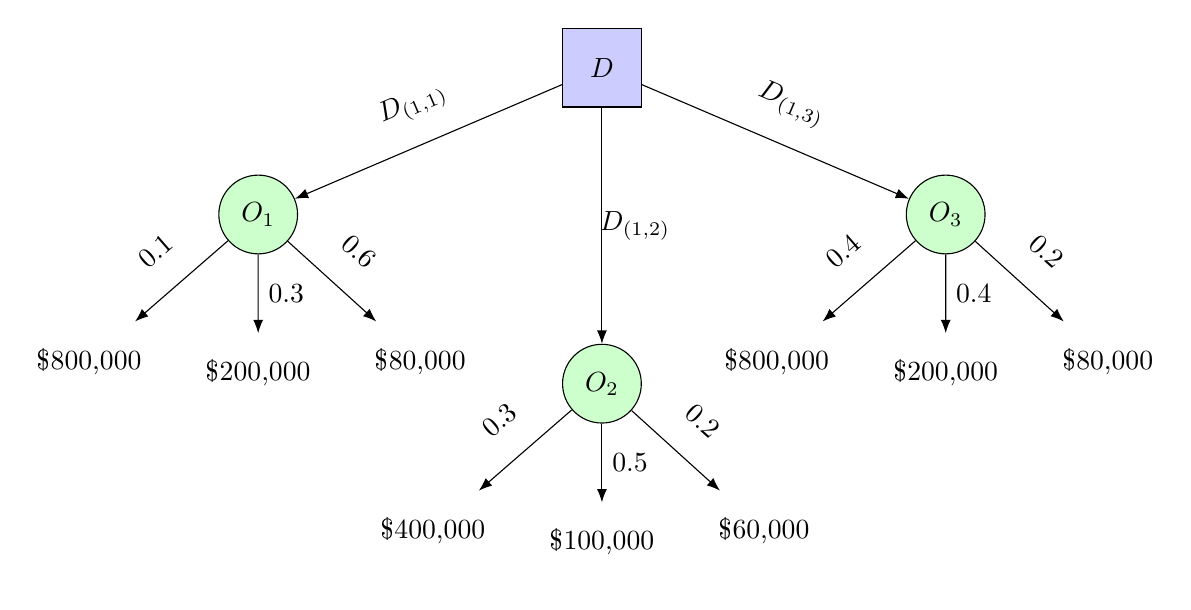
\begin{tikzpicture}[
                scale = 0.3,
                every node/.style={minimum width=1cm,minimum height=1cm},
                decision/.style={rectangle, draw, fill=blue!20},
                chance/.style={circle, draw, fill=green!20},
                outcome/.style={},
                line/.style={-Latex}
            ]
            \node[decision] (D) {$D$};
            \node[chance, below left=1cm and 3.5cm of D] (O1) {$O_1$};
            \node[chance, below=3cm of D] (O2) {$O_2$};
            \node[chance, below right=1cm and 3.5 cm of D] (O3) {$O_3$};
            
            \draw[line] (D) -- node[above, sloped] {$D_{(1,1)}$} (O1);
            \draw[line] (D) -- node[above, sloped] {$D_{(1,3)}$} (O3);
            \draw[line] (D) -- node[right = -0.15] {$D_{(1,2)}$} (O2);
            
            \node[outcome, below left=of O1] (R1) {\$800,000};
            \node[outcome, below=of O1] (R2) {\$200,000};
            \node[outcome, below right=of O1] (R3) {\$80,000};
            \draw[line] (O1) -- node[above, sloped] {0.1} (R1);
            \draw[line] (O1) -- node[right = -0.15] {0.3} (R2);
            \draw[line] (O1) -- node[above, sloped] {0.6} (R3);
            
            \node[outcome, below left=of O2] (B1) {\$400,000};
            \node[outcome, below=of O2] (B2) {\$100,000};
            \node[outcome, below right=of O2] (B3) {\$60,000};
            \draw[line] (O2) -- node[above, sloped] {0.3} (B1);
            \draw[line] (O2) -- node[right = -0.15] {0.5} (B2);
            \draw[line] (O2) -- node[above, sloped] {0.2} (B3);
            
            \node[outcome, below left=of O3] (T1) {\$800,000};
            \node[outcome, below=of O3] (T2) {\$200,000};
            \node[outcome, below right=of O3] (T3) {\$80,000};
            \draw[line] (O3) -- node[above, sloped] {0.4} (T1);
            \draw[line] (O3) -- node[right = -0.15] {0.4} (T2);
            \draw[line] (O3) -- node[above, sloped] {0.2} (T3);
        \end{tikzpicture}
        }\\
        
        where:
        \begin{center}
            \begin{tabular}{l l}
                $D:$ & Decision Node\\
                $D_{(1,1)}:$ & Build New Product, Rapid Development\\
                $D_{(1,2)}:$ & Strengthen Existing Products\\
                $D_{(1,3)}:$ & Build New Product, Thorough Development\\
                $O_1:$ & Well $(P=0.1)$, Moderate $(P=0.3)$, Poor $(P=0.3)$\\
                $O_2:$ & Well $(P=0.3)$, Moderate $(P=0.5)$, Poor $(P=0.2)$\\
                $O_3:$ & Well $(P=0.4)$, Moderate $(P=0.4)$, Poor $(P=0.2)$
            \end{tabular}
        \end{center}
        
        \item The expected payoff of each choice is computed below along with a description of the optimal strategy.
        \begin{align*}
            D_{(1,1)} &= (0.1 \cdot \$800{,}000) + (0.3 \cdot \$200{,}000) + (0.6 \cdot \$80{,}000) - \$120{,}000 \\
            &= \$68{,}000 \\ \\
            D_{(1,2)} &= (0.3 \cdot \$400{,}000) + (0.5 \cdot \$100{,}000) + (0.2 \cdot \$60{,}000) - \$100{,}000 \\
            &= \$82{,}000 \\ \\
            D_{(1,3)} &= (0.4 \cdot \$800{,}000) + (0.4 \cdot \$200{,}000) + (0.2 \cdot \$80{,}000) - \$300{,}000 \\
            &= \$116{,}000
        \end{align*}
        
        \textbf{Optimal Strategy:} Build New Product, Thorough Development ($D_{(1,3)}$ = \$116{,}000)\\
    \end{enumerate}
    
    \item Harry is in his last semester at Cornell and is thinking about taking SYSEN 5200 before graduating. He has a decision to make:
    \begin{enumerate}
        \item enroll now
        \item take another course instead
        \item delay enrollment until he gets his first prelim grades back
    \end{enumerate}

    If he enrolls and passes the course, he estimates his starting salary will increase by $x = \$30,000$. If he enrolls but fails, he will need to stay at Cornell for another semester with a tuition cost of \$25,000. If he chooses to delay his decision but ends up not taking the course, he will have missed the opportunity to take another course that is of interest and will need to take it online at a cost of \$5,000.

    Judging from his knowledge in probability and statistics, Harry estimates that he can pass the course with probability $p = 0.6$. Based on previous years’ statistics, out of the students who passed, 0.8 fraction got a good grade on the first prelim, i.e. $P(\text{good grade on prelim } $|$ \text{ pass}) = 0.8$. On the other hand, out of the students who failed the course, 0.9 fraction got a bad grade on the first prelim, i.e. $P(\text{bad grade on prelim } $|$ \text{ fail}) = 0.9$. For simplicity, assume that Harry cannot drop the class once enrolled.

\break
    \begin{enumerate}
        \item The following exhibits the decision tree with labeled nodes, classified by type, including the outcomes and their respective probabilities.\\
        
        \resizebox{\linewidth}{!}{
            \begin{tikzpicture}[scale = 0.3, every node/.style={minimum width=1cm,minimum height=1cm}, decision/.style={rectangle, draw, fill=blue!20}, chance/.style={circle, draw, fill=green!20}, outcome/.style={}, line/.style={-Latex}]
            
            \node[decision] (D) {$D_{1}$};
            \node[chance, below left=1cm and 3.5cm of D] (O1) {$O_1$};
            \node[chance, below=1cm of D] (O2) {$O_2$};
            \node[chance, below right=1cm and 3.5 cm of D] (O3) {$O_3$};
            \node[decision, below left=1cm and 1cm of O3] (D2) {$D_{2}$};
            \node[decision, below right=1cm and 1cm of O3] (D3) {$D_{3}$};
            
            \draw[line] (D) -- node[above, sloped] {$D_{(1,1)}$} (O1);
            \draw[line] (D) -- node[above, sloped] {$D_{(1,3)}$} (O3);
            \draw[line] (D) -- node[right = 0] {$D_{(1,2)}$} (O2);
            
            \node[outcome, below left=of O1] (R1) {\$30,000};
            \node[outcome, below right=of O1] (R3) {-\$25,000};
            \draw[line] (O1) -- node[above, sloped] {0.6} (R1);
            \draw[line] (O1) -- node[above, sloped] {0.4} (R3);
            
            \node[outcome, below=of O2] (B2) {\$0};
            \draw[line] (O2) -- node[right = -0.15] {1.0} (B2);
            \draw[line] (O3) -- node[above, sloped] {0.52} (D2);
            \draw[line] (O3) -- node[above, sloped] {0.48} (D3);
            
            \node[chance, below left=1cm and 1cm of D2] (T1) {$O_4$};
            \draw[line] (D2) -- node[above, sloped] {$D_{(2,1)}$} (T1);
            \node[outcome, below right=of D2] (E2) {-\$5,000};
            \draw[line] (D2) -- node[above, sloped] {$D_{(2,2)}$} (E2);
            \node[outcome, below left=of D3] (E3);

            \node[chance, below right=1cm and 1cm of D3] (U1) {$O_5$};
            \draw[line] (D3) -- node[above, sloped] {$D_{(3,2)}$} (U1);
            \node[outcome, below left=of D3] (E3);
            \draw[line] (D3) -- node[above, sloped] {$D_{(3,1)}$} (E3);
            \node[outcome, below left=of U1] (S4) {\$30,000};
            \node[outcome, below right=of U1] (S5) {-\$25,000};
            \draw[line] (U1) -- node[above, sloped] {0.1} (S4);
            \draw[line] (U1) -- node[above, sloped] {0.9} (S5);
            
            \node[outcome, below left=of T1] (R4) {\$30,000};
            \node[outcome, below right=of T1] (R5) {-\$25,000};
            \draw[line] (T1) -- node[above, sloped] {0.8} (R4);
            \draw[line] (T1) -- node[above, sloped] {0.2} (R5);
            \end{tikzpicture}
        }

        where:
        \begin{center}
            \begin{tabular}{l l}
                $D:$ & Decision Node\\
                $D_{(1,1)}:$ & Enroll Now\\
                $D_{(1,2)}:$ & Take Another Course\\
                $D_{(1,3)}:$ & Delay Enrollment\\
                $D_{(2,1)}:$ & Enroll in Course\\
                $D_{(2,2)}:$ & Take Online Course\\
                $D_{(3,1)}:$ & Take Online Course\\
                $D_{(3,2)}:$ & Enroll in Course\\
                $O_1:$ & Pass $(P=0.6)$, Fail $(P=0.4)$\\
                $O_2:$ & Abandon $(P=1.0)$\\
                $O_3:$ & Pass $(P=0.52)$, Fail $(P=0.48)$\\
                $O_4:$ & Pass $(P=0.8)$, Fail $(P=0.2)$\\
                $O_5:$ & Pass $(P=0.1)$, Fail $(P=0.9)$
            \end{tabular}\\~\\
        \end{center}
        
        \item The probabilities for all outcomes based on the information given above can be computed as such:\\

        $D_{(1,1)}$:
        \begin{align*}
            P(\text{pass}) &= 0.6 \\
            P(\text{fail}) &= 0.4
        \end{align*}
        
        $D_{(1,2)}$:
        \begin{align*}
            P(\text{abandon}) = 1.0
        \end{align*}
        
        $D_{(1,3)}$:\\
        
        We first compute $P(\text{good grade})$ using the law of total probability:
        \begin{equation}
            \begin{split}
                P(\text{good grade}) &= P(\text{good grade } | \text{ pass}) \cdot P(\text{pass}) + P(\text{good grade } | \text{ fail}) \cdot P(\text{fail})\\
                &= 0.8 \cdot 0.6 + 0.1 \cdot 0.4\\
                &= 0.52
            \end{split}
        \end{equation}
            
        Then we have:
         \begin{equation}
             \begin{split}
                P(\text{pass $|$ good grade}) &= \frac{P(\text{good grade $|$ pass})\cdot P(\text{pass})}{P(\text{good grade})}\\
                &= \frac{0.8 \cdot 0.6}{0.52}\\
                &= 0.923
             \end{split}
        \end{equation}

        \begin{equation}
            \begin{split}
                P(\text{fail $|$ good grade}) &= 1 - P(\text{pass $|$ good grade})\\
                &= 1 - 0.923\\
                &= 0.077 \\  
            \end{split}
        \end{equation}
        
        To calculate $P(\text{bad grade})$ using the law of total probability:

        \begin{equation}
            \begin{split}
                P(\text{bad grade}) &= P(\text{bad grade } | \text{ pass}) \cdot P(\text{pass}) + P(\text{bad grade } | \text{ fail}) \cdot P(\text{fail})\\
                &= 0.2 \cdot 0.6 + 0.9 \cdot 0.4\\
                &= 0.12 + 0.36\\
                &= 0.48
            \end{split}
        \end{equation}

        Then we have:
        \begin{equation}
            \begin{split}
              P(\text{pass $|$ bad grade}) &= \frac{P(\text{bad grade $|$ pass}) \cdot P(\text{pass})}{P(\text{bad grade})}\\
              &= \frac{0.2 \cdot 0.6}{0.48}\\
              &= 0.25
            \end{split}
        \end{equation}

        Finally:
        \begin{equation}
            \begin{split}
              P(\text{fail $|$ bad grade}) &= 1 - P(\text{pass $|$ bad grade})\\
              &= 1 - 0.25\\
              &= 0.75
            \end{split}
        \end{equation}
        
        where good grades and bad grades describe previous years' prelim.\\~\\
                
        \item The expected values for each decision node can be computed such that:
        \begin{equation}
            \begin{split}
                D_{(1,1)} &= (0.6 \cdot \$30{,}000) + (0.4 \cdot -\$25{,}000)\\
                &= \$18{,}000 - \$10{,}000\\
                &= \$8{,}000\\~\\
                D_{(1,2)} &= \$0\\~\\
                D_{(1,3)} &= (0.52 \cdot \$19{,}000) + (0.48 \cdot -\$5,000)\\
                &= \$9,880 - \$2,400\\
                &= \$7,480
            \end{split}
        \end{equation}
        
        where:
        \begin{equation}
            \begin{split}
                D_{(2,1)} &= (0.8 \cdot \$30{,}000) + (0.2 \cdot -\$25{,}000)\\
                &= \$24{,}000 - \$5{,}000\\
                &= \$19{,}000\\~\\
                D_{(2,2)} &= -\$5{,}000\\~\\
                D_{(3,1)} &= -\$5{,}000\\~\\
                D_{(3,2)} &= (0.1 \cdot \$30{,}000) + (0.9 \cdot -\$25{,}000)\\
                &= \$3{,}000 - \$22{,}500\\
                &= -\$19{,}500
            \end{split}
        \end{equation}
        
        \textbf{Optimal Strategy:} Enroll Now ($D_{(1,1)}$ = \$8,000)\\
            
        \item The minimum value of $x$ for Harry to be willing to enroll immediately is the expected value of enrolling now, which can be expressed as:\\

        \begin{equation}
            \$7{,}480 + 0.6x - 0.4 \cdot \$25,000
        \end{equation}

        Now, we solve for $x$:
        \begin{equation}
            \begin{split}
                \$8{,}000 &\geq \$7{,}480 + 0.6x - 0.4 \cdot \$25{,}000\\
                \$8{,}000 &\geq \$7{,}480 + 0.6x - \$10{,}000\\
                \$11{,}520 &\geq 0.6x\\
                x &\geq \$19{,}200
            \end{split}
        \end{equation}
            
        Therefore, the minimum value of $x$ for Harry to be willing to enroll immediately is \$19,200.
    \end{enumerate}

%% end
\end{enumerate}
\end{document}